\documentclass{iopart}
% only packages used
%\usepackage{amsfonts}
%\usepackage{amsmath}
%\usepackage{showkeys}
\usepackage{graphicx}
\usepackage{hyperref}
%\usepackage{multicol}
%\input{definitions}

%some abb:
\newcommand{\sinc}{sinc}
\usepackage[utf8]{inputenc}
\newcommand{\nota}[1]{{\bf\tiny #1}}
\DeclareGraphicsRule{*}{mps}{*}{}
\begin{document}
\title{NONLOCAL OPTICAL RESPONSE OF LAYERED SYSTEMS}
\author{J.S. P\'erez-Huerta$^{1}$, W. Luis Moch\'an$^2$}%00, Guillermo
%  P. Ortiz$^3$, and Bernardo S. Mendoza$^4$} 
\address{$^1$ Unidad
  Académica de Física, Universidad Autónoma de Zacatecas, Calzada
  Solidaridad Esquina con Paseo La Bufa S/N, Zacatecas
  México. \\ $^2$Instituto de Ciencias F\'{\i}sicas, Universidad
  Nacional Aut\'onoma de M\'exico, Apartado Postal 48-3, 62251
  Cuernavaca, Morelos, M\'exico.\\
%% \\ $^3$Departamento de F\'isica,
%%   Facultad de Cs. Exactas, Naturales y Agrimensura, Universidad
%%   Nacional del Nordeste, Av. Libertad 5400 Campus-UNNE, W3404AAS
%%   Corrientes, Argentina.\\ $^4$Division of Photonics, Centro de
%%   Investigaciones en Optica, \\Le\'on, Guanajuato, M\'exico.\\ 
  E-mail:
  jsph: {\tt jsperez@fisca.uaz.edu.mx}, wlmb: {\tt mochan@fis.unam.mx}}
% gpo: {\tt gortiz@exa.unne.edu.ar}, bsm: {\tt bms@cio.mx} }
%

\begin{abstract}
We propose an analytical procedure for the calculation of the
macroscopic dielectric response of one dimensional periodic systems
made of two alternated materials, each of them characterized by a well
defined dielectric function which may make up by arbitrary material,
and it could has a complex function of the frequency. We introduce an
external electric current to excite the system and we solve the exact
wave equation for the electromagnetic field subject to the appropriate
boundary conditions. Then we eliminate the spatial fluctuations to
obtain the macroscopic field. From the macroscopic wave equation we
find the the macroscopic dielectric response for each polarization
direction of the electric current.
\end{abstract}

%---------------------------------------------------------
\section{Introduction}
FALTA JUSTIFICACION

%% In this paper we obtain

%% The paper is organized as follows: 
%% In Sec. \ref{Theory} we develop our general 
%% theoretical formulation of the macroscopic electric response 
%% of one dimensional systems. In Sec. \ref{binary} we adapt our
%% formulation to periodic systems made of two alternating materials with
%% well defined dielectric functions. 
%% In Sec. \ref{Numeric} we apply our formalism to a 1D photonic crystal
%% made up of non-dispersive dielectric components and we obtain its
%% non-local macroscopic dielectric tensor and its full band
%% structure. Finally, in Sec.~\ref{conclusion} we present our conclusions.

%---------------------------------------------------------
\section{One dimensional system}
\label{Theory}

Consider a non-magnetic one dimensional periodic system which is
invariant along cartesian directions $x$ and $y$, made of two
materials $A$ and $B$ with dielectric functions $\epsilon_A$ and
$\epsilon_B$. We suposse that both media are local and isotropic,
therefore both dielectric functions are simply complex functions of
the frequency. The material $A$ fills the region between $0\le z \le
L_A$ while material $B$ fills the region $L_A\le z\le L$. So that the
length of the unit cell is $L=L_A+L_B$ and we repeat it periodically,
as we show in Fig. \ref{1Dsys}. 


We imposse an external electric current densitry
$\mathbf{J}=(J_x,0,J_z)$ into the system. We asumme this current as a
propagating armonic wave traveling acroos the structure with direction
given by the wavevector $\mathbf K$.  In Fig. Right \ref{fig:Eps_M_L1L2} we 
show this configuration.
\section{LAYERED SYSTEMS}
\begin{figure}
  \begin{minipage}{0.5\textwidth}
  \centering
  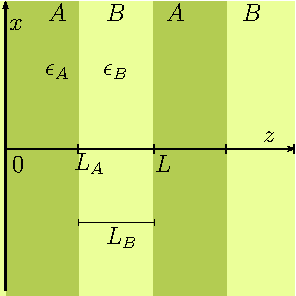
\includegraphics[scale=1]{1Dfronteras-pics}
  \end{minipage}
  \begin{minipage}{0.5\textwidth}
    \centering
    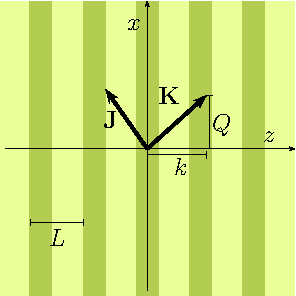
\includegraphics[scale=1]{red1d-pics}
  \end{minipage}
  \caption{Panel izquierdo: Sistema en una dimensión que consiste en
    películas de cierto material con respuesta dieléctrica
    $\epsilon_A$ y ancho $L_A$ alternadas periódicamente con películas
    de otro medio con respuesta dieléctrica $\epsilon_{B}$ y ancho
    $L_B$. Se muestran las coordenadas de las algunas interfaces y el
    periodo $L$ de la red. Panel derecho: Se muestra la estructura y
    el sistema coordenado, así como la corriente externa $\mathbf J$ y
    su vector de onda $\mathbf k$.}
  \label{1Dsys}
\end{figure}
\section{Wave equation}
Nuestro objetivo es encontrar cómo responde el sistema a esta
corriente. Para ello, hallaremos el campo eléctrico microscópico
producido por esta corriente resolviendo la ecuación de onda con
fuentes en cada una de las regiones y exigiendo que la solución
obtenida cumpla con las condiciones de contorno correspondientes a
cada una de las interfaces. Al ser un sistema periódico, ésta solución
deberá de ser una onda de Bloch con vector de Bloch $\mathbf k$. Una
vez conocido el campo microscópico, podemos extraer de él la
componente macroscópica para finalmente obtener la respuesta
macroscópica del sistema mediante la relación constitutiva asociada a
dicho campo.

Escribimos la dependencia espacial de la corriente externa como
$\mathbf J =(J_x, 0, J_z)e^{i(kz+Qx)}$, con $J_x$, $J_z$ las
componentes cartesianas de la amplitud de la corriente externa, $k$ es
la componente $z$ del vector de onda y $Q$ la componente $x$. La
ecuación de onda inhomogénea en la región $\alpha=A,B$ es simplemente
\begin{equation}
  \label{Eonda}
  \left(\nabla\times\nabla\times-\frac{\omega^2}{c^2}\epsilon_\alpha
  \right) \mathbf E = \frac{4 \pi i\omega}{c^2}\mathbf J,
\end{equation}
que son dos ecuaciones diferenciales acopladas para las componentes
cartesianas del campo eléctrico. Debido a la simetría translacional en
la dirección $x$, suponemos que el campo eléctrico tiene la forma
\begin{equation}
  \label{efield}
\mathbf E^{\alpha}(x,z) =( E_{x}^{\alpha}(z), 0, E_{z}^{\alpha}(z))e^{iQx},
\end{equation}
entonces, la ec. de onda es
\begin{eqnarray}  \label{onda2}
\frac{\partial}{\partial z}\left(i Q
E_{z}^{\alpha}-\frac{\partial}{\partial z} E_{x}^{\alpha}\right)
-\frac{\omega}{c}\epsilon_{xx}^{\alpha}E_{x}^{\alpha}&=& \frac{4 \pi
  i\omega}{c^2}J_xe^{ikz},\\-i Q\left(i Q E_{z}^{\alpha}-\frac{\partial}{\partial
  z} E_{x}^{\alpha}\right)
-\frac{\omega}{c}\epsilon_{zz}^{\alpha}E_{z}^{\alpha}&=& \frac{4 \pi
  i\omega}{c^2}J_ze^{ikz},
\end{eqnarray}
La solución general de las ecs. \ref{onda2} es la superposición de una
solución particular de las ecuaciones inhomogéneas mas la solución
general de las correspondiente ecuación de onda homogénea. Entonces,
la parte del campo eléctrico microscópico que depende de $z$ en las
dos regiones contenidas en el intervalo $0\le z\le L$ está dado por
\begin{equation}
\label{Emicro1d}
  E^{\alpha}_i(z) ={ E^{\alpha}_0}_{i}e^{ikz}+
  {E^{\alpha}_{D}}_{i}e^{ik_{\alpha}z}+  {E^{\alpha}_{I}}_{i}e^{-ik_{\alpha}z},
\end{equation}
para $i=x,z$ y donde hemos introducido el número de onda libre en la
región $\alpha$,
\begin{equation}
\label{kmicro1d}
  k_{\alpha}^2=\epsilon_{\alpha}q^2,
\end{equation}
también ${E^{\alpha}_{\beta}}_{i}$ con $\beta=0,D,I$ son doce
coeficientes por determinar correspondiendo a ondas libres que corren
hacia la derecha ($D$) o hacia la izquierda ($I$) en el medio
$\alpha$.  Los coeficientes ${E^{\alpha}_{0}}_{i}$ corresponde a una
onda forzada que se propaga con el mismo vector de onda $\mathbf k$
que la corriente externa, y se obtienen al sustituir esta solución
forzada en la ecuación inhomogénea. La componente catesiana $z$ del
campo eléctrico que depende de $z$ se puede obtener mediante la
componente cartesiana $x$ del campo como
\begin{equation}
\label{ez}
E^{\alpha}_{z}=\frac{iQ}{q^2\epsilon^{\alpha}_{zz}-Q^2}\frac{\partial
  E^{\alpha}_{x}} {\partial z},
\end{equation}
por lo que sólo es necesario determinar los cuatro coeficientes para
la componente $x$ del campo eléctrico.

De manera análoga, podemos escribir la componente $y$ del campo
magnético microscópico $B^\alpha(z)$ dentro del medio $\alpha$ y
expresarla en términos de las componentes del campo eléctrico
mediante la ley de Faraday como,
\begin{equation}
\label{Bmicro1d}
 B^{\alpha}(z) =\frac{c}{i\omega} \left(\frac{\partial
  E^{\alpha}_{x}} {\partial z}-iQ E^{\alpha}_{z} \right),
\end{equation}
qu es la única componente no nula del campo magnético. Las condiciones
de continuidad para la componente tangencial del campo eléctrico y del
campo magnético en las fronteras $z=L_A$ y $L$ están dadas por los
límites \numparts
\begin{eqnarray}
  \label{CCA1} 
  E^{A}_x(z\to L_A^-)&=&  E_x^{B}(z\to L_A^+),\\
  \label{CCA2}
  B^{A}(z\to L_A^-)&=&  B^{B}(z\to L_A^+),\\
  \label{CCB1}
  E_x^{A}(z\to L^+)&=&  E_x^{B}(z\to L^-),\\
  \label{CCB2}
  B^{A}(z\to L^+)&=&  B^{B}(z\to L^-),
\end{eqnarray} 
\endnumparts
%% \end{subequations}
donde los superíndices $\pm$ indican si nos acercamos a la superficie
por la derecha ($+$) o por la izquierda ($-$). Notamos que las
ecs. \ref{Emicro1d} describen al campo únicamente en el intervalo
$0\le z\le L$, por lo cual no podemos emplearla en el lado derecho de
las ecs. \ref{CCB1} y \ref{CCB2}. Sin embargo, el teorema de Bloch
nos dice que al avanzar un periodo $L$ hacia la derecha, todos los
campos adquieren simplemente una fase,
 \numparts
\begin{eqnarray}
  E_x^{A}(z\to L^+)&=&  E_x^{A}(z\to 0^+)e^{ikL},\\
  B^{A}(z\to L^+)&=&  B^{B}(z\to 0^+)e^{ikL}.
\end{eqnarray}
 \endnumparts
lo cual nos permite cerrar el sistema de ecuaciones
\ref{CCA1}-\ref{CCB2}. Sustituyendo en ellas la ec. \ref{Emicro1d},
\ref{ez}, \ref{Bmicro1d}, las expresamos como cuatro ecuaciones
inhomogéneas acopladas con cuatro incógnitas, las cuales escribimos
como
\begin{eqnarray}
%% \label{inhomosys}
%\label{MWaveMatrix}
\left(
\begin{array}{cccc}
e^{ik_{A}L_A}&-e^{ik_{B}L_A}&e^{-ik_{A}L_A}&-e^{-ik_{B}L_A}\\
\eta_Ak_Ae^{ik_AL_A}&-\eta_Bk_Be^{ik_{B}L_A}&-
\eta_Ak_Ae^{-ik_{A}L_A}&+\eta_Bk_Be^{-ik_{B}L_A}\\
1&-e^{i(k_{B}-k)L}&1&-e^{-i(k_{B}+k)L}\\
\eta_Ak_A&-\eta_Bk_Be^{i(k_{B}-k)L}&-\eta_Ak_A&\eta_Bk_Be^{-i(k_{B}+k)L}
\end{array}
\right) \times  &\\
\left(
\begin{array}{c}
 {E^{A}_{D}}_{x}\\
 {E^{B}_{D}}_{x}\\
 {E^{A}_{I}}_{x}\\
 {E^{B}_{I}}_{x}
\end{array}
\right)=
\left(
\begin{array}{c}
\Delta E_0  e^{ikL_A}\\
k e^{ikL_A}(\eta_B{E^{B}_{0}}_{x}-\eta_A{E^{A}_{0}}_{x})\\
\Delta E_0  \\
k(\eta_B{E^{B}_{0}}_{x}-\eta_A{E^{A}_{0}}_{x})\\
\end{array}
\right)&
\end{eqnarray}
donde $\Delta E_0 ={E_{0}^B}_{x}-{E_{0}^A}_{x}$. 

El campo eléctrico, siendo una onda de Bloch, no es una función
periódica en $z$, pero $\mathbf{E} e^{-ikz}$ sí lo es. Entonces podemos
expandir esta función como una serie de Fourier
\cite{spiegel1974fourier} cuyos coeficientes son
\begin{equation}  \label{EG1}
\mathbf{E} _{ G}=\frac{1}{L} \left(
\begin{array}{c}
\int_{0}^{L}  E_x (x,z)e^{-i(k + G)z}dz\\
0\\
\int_{0}^{L}  E_z (x,z)e^{-i(k + G)z}dz
\end{array}\right)
\end{equation}
Identificamos el campo eléctrico macroscópico como el término $G=0$ de
dicha serie de Fourier, $\mathbf{E}^M(z)\equiv \mathbf{E} _{G=0}
e^{ikz}$. Del análogo macrosópico de la ec. \ref{Eonda}, tenemos que
\begin{equation}\label{EMacro1d}
 \mathbf{E}^M = \frac{4 \pi}{i\omega} {\mathcal
   W}^{-1}_{M}\mathbf{J}^M,
\end{equation}
con ${\mathcal W}^{-1}_{M}=...$. Como nosotros podemos fijar la
corriente externa y calcular el campo eléctrico macroscópico
correspondiente, se pueden determinar las componentes cartesianas del
tensor ${\mathcal W}^{-1}_{M}$, al variar para las diferentes
orientaciones del vector polarización de la corriente eléctrica y
resolver las ecuaciones para todas las componentes cartesianas de
${({\mathcal W}^{-1}_{M})}_{ij}$. Finalmente, haciendo una inversión
matricial de este tensor macroscópico se puede calcular el tensor
dieléctrico macroscópico
\begin{equation}
  \label{EpsMacroTensor}
  \epsilon^M_{ij}(\omega,\mathbf k)=
  \frac{1}{q^2}(K^2\delta_{ij}- K_i  K_j)+\mathcal W^M_{ij}(\omega,
  \mathbf K),
\end{equation}
qu es la respuesta dieléctrica del sistema estructurado.


El resultado \ref{epszz} para la función macroscópica es exacto en
el sentido que no se ha realizado ninguna aproximación para obtenerlo
y es analítico al estar en términos de funciones analíticas y de la
solución de un sistema de ecuaciones pequeño que puede resolverse
explícitamente, aunque las expresiones resultantes sean tediosas.  La
respuesta macroscópica \ref{epszz} es explícitamente una función del
vector de onda $k$ además de ser una función de la frecuencia
$\omega$. Debemos notar que las amplitudes $E^{\alpha}_{\beta}(z)$
dependen también de $k$ y $\omega$.


%% \begin{equation}  \label{epszz}
%% \begin{split}
%% \epsilon^M(\omega,k) = (kc/\omega)^2 +\frac{4 \pi
%%   J_0L}{i\omega}/&(L_{A}E^{A}_0+L_{B}E^{B}_0 \\ &
%% +E^{A}_{D}L_{A}\sinc((k_{A}-k)L_{A}/2)e^{i(k_{A}-k)L_{A}/2} \\ & +
%% E^{A}_{I}L_{A}\sinc((k_{A}+k)L_{A}/2)e^{-i(k_{A}+k)L_{A}/2} \\ & +
%% E^{B}_{D}L_{B}\sinc((k_{B}-k)L_{B}/2)e^{i(k_{B}-k)L_{B}/2} \\ & +
%% E^{B}_{I}L_{B}\sinc((k_{B}+k)L_{B}/2)e^{-i(k_{B}+k)L_{B}/2}),
%% \end{split}
%% \end{equation}

\section{Elser's Formule vs our results}
En el trabajo de[elser], derivan una fómula para la respuesta efectiva
que depende tanto de la frecuencia como del vector de onda 

FALTA





\section{Results}
\label{Numeric}
%\subsection{Numerical macroscopic optical responses}

To test our formalism, 

FALTA


\begin{figure} \centering
  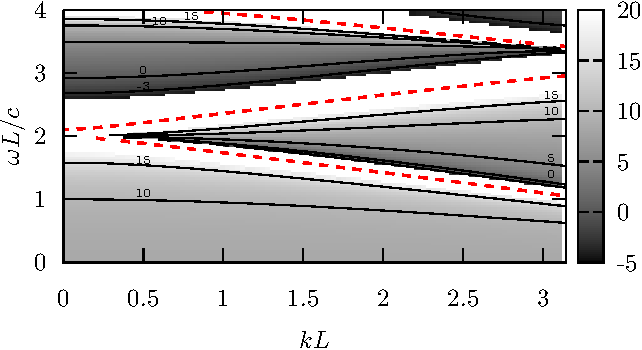
\includegraphics{1D_epszz_epsa_16_epsb_1_f_05map}
\caption{Respuesta dieléctrica macroscópica
  $\epsilon^M(\omega,k)$ del sistema periódico unidimensional mostrado
  en la figura \ref{1Dsys} con $\epsilon_A=1$, $\epsilon_{B}=12$ y
  $f_{A}=f_{B}=0.5$ como función de la frecuencia normalizada
  $\omega L/c$ y del vector de onda normalizado $kL$. Se muestran
  algunos contornos a lo largo de los cuales $\epsilon^M$ es constante
  (líneas
  sólidas) y las posiciones de los polos (líneas a trazos). Las
  regiones blancas corresponden a valores fuera del rango
  $\sim(-5,15)$  elegido para obtener un contraste adecuado en la
  representación mediante tonos de grises.
}
\label{Fepszz}
\end{figure}



%% \begin{figure} 
%%   \includegraphics{primerabanda_compara}
%% \caption{.
%% }
%% \label{primera}
%% \end{figure}



\begin{figure}
\centering
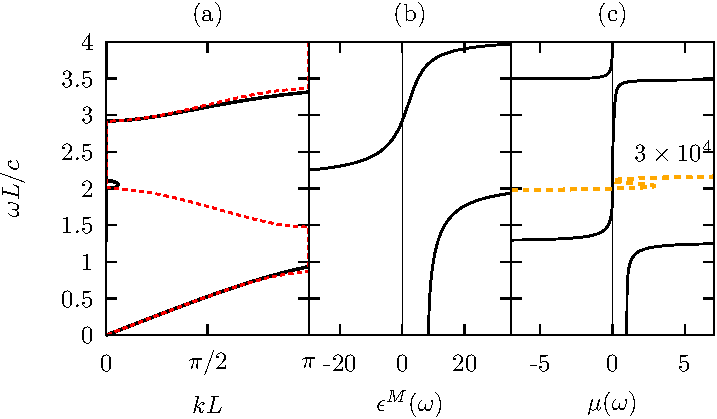
\includegraphics{bandas_locales_1D}
\caption{(a) Relación de dispersión local para el mismo sistema
  mostrado en la figura \ref{1Dsys} (línea sólida) obtenida de la ec.
  \ref{local1d} y relación de dispersión exacta (línea a
  trazos). (b) Función dieléctrica macroscópica local 
  $\epsilon^M(\omega)$.  (c) Respuesta macroscópica magnética
  $\mu(\omega)$ (línea solida) y detalle escalado $3\times
  10^4\mu(\omega)$ veces (línea a trazos y puntos azul).}
\label{1d:localbanda}
\end{figure}



\section{Conclusions}
\label{conclusion}
 We obtained analytically the macroscopic dielectric function.
 Retardation yields spatial, as well as temporal dispersion.
 Our macroscopic formulation yields the exact photonic band
  structure of the system.
 Spatial dispersion yields magnetic response in a local
  approximation.
 Singularity structure produces artifacts in approximate band structure. 
 We identified the non-local dielectric function from the response
  to external excitations; the dispersion relation \cite{Elser07}
  is not enough to obtain the correct $\epsilon^M(k,\omega)$ for
  arbitrary  $k$ and $\omega$. 

%---------------------------------------------------------
%\section{Results}
%\label{Numeric}



%\section{Conclusions}



\ack J.S.P.H. wishes to acknowledge
\section*{References} 
% ----------------------------------------------------------------\cite{}
\bibliographystyle{unsrt}%amsplain
\bibliography{Haydockbib}
%---------------------------------------------------------
\appendix 

\section{Deduccion de Fórmulas}
\label{AppendixA}
De

\end{document}

\begin{thebibliography}{10}
\bibitem{JPerez2013}
{\small
J S P{\'e}rez-Huerta, Guillermo P. Ortiz, S. Mendoza, and W. Luis Moch{\'a}n.
%\newblock Macroscopic optical response and photonic bands
\newblock {\em New Journal of Physics}, 15(4):043037, 2013.


\bibitem{Elser07}
Justin Elser, Viktor~A. Podolskiy, Ildar Salakhutdinov, and Ivan Avrutsky.
%\newblock Nonlocal effects in effective-medium response of nanolayered
%  metamaterials.
\newblock {\em Applied Physics Letters}, 90(19):191109, 2007.}
\end{thebibliography}
